\chapter{Implementation}
\label{ch:implementation}

\section{Overview and design goals}
\label{sec:impl-overview}

The project is deliberately split into two parts: \pkg{}, a library published on PyPI that
turns a string into a list of chunks, and everything under \code{app/} and
\code{eval/}, the evaluation harness that produces the results of
\cref{ch:evaluation}. The split ensures that a user of the library does not have to
install anything besides the chunker itself, and the packaging configuration enforces it.
The library has three runtime dependencies: an HTTP client, a sentence tokeniser and a
language detector. A vector store, a PDF reader and the two framework adapters for
LangChain and LlamaIndex are optional extras.

\paragraph{Hardware constraints.} Several design decisions follow from the hardware the
project was developed and evaluated on: a MacBook Air with an M1 chip and
\SI{8}{\giga\byte} of memory. Three processes have to be active during an entire
evaluation run: Ollama running \code{qwen3.5:4b} for the boundary decisions (about
\SI{3.5}{\giga\byte}, largely wired and therefore not swappable), Ollama serving bge-m3 for
the embeddings (about \SI{1.2}{\giga\byte}) and the Python process holding the chunks and
the vector store (\SIrange{0.5}{1.5}{\giga\byte}). As a consequence, free memory fell below
\SI{60}{\mega\byte} for extended periods and the swap file grew to \SI{15}{\giga\byte}.

Two design decisions follow directly from these constraints. First, embeddings are
computed by a second Ollama-served model rather than in-process, so that no PyTorch
runtime occupies additional memory in the Python process. Second, chunking and evaluation
are split into two phases with a persistent cache between them: chunking a document is
far slower on this hardware than evaluating the chunks, and the cache ensures that an
interruption does not destroy completed chunking work. \Cref{sec:harness}
describes what the cache records and why.

\paragraph{Scope.} The library implements chunking only and deliberately leaves out
reranking, query expansion, hybrid retrieval and similar components. These belong to the
retrieval stage and could raise the hit rates, but the improvement would not come from the
chunking and would distort the comparison with the baseline strategies. Whether the effect
of LLM-based chunking persists with a stronger retrieval stage is a worthwhile question,
but it is outside the scope of this work.

\section{Architecture}
\label{sec:architecture}

The project is designed so that each stage of the chunking and of its post-processing can
be replaced without affecting the others. The LLM client is therefore defined by a
structural protocol: any object with a \code{chat(messages)} method can be used, which
removes the hard dependency on Ollama. The prompts are dataclasses that can be substituted,
and the post-processors share a common interface, so that they can be used
interchangeably.

\begin{figure}[htbp]
  \centering
  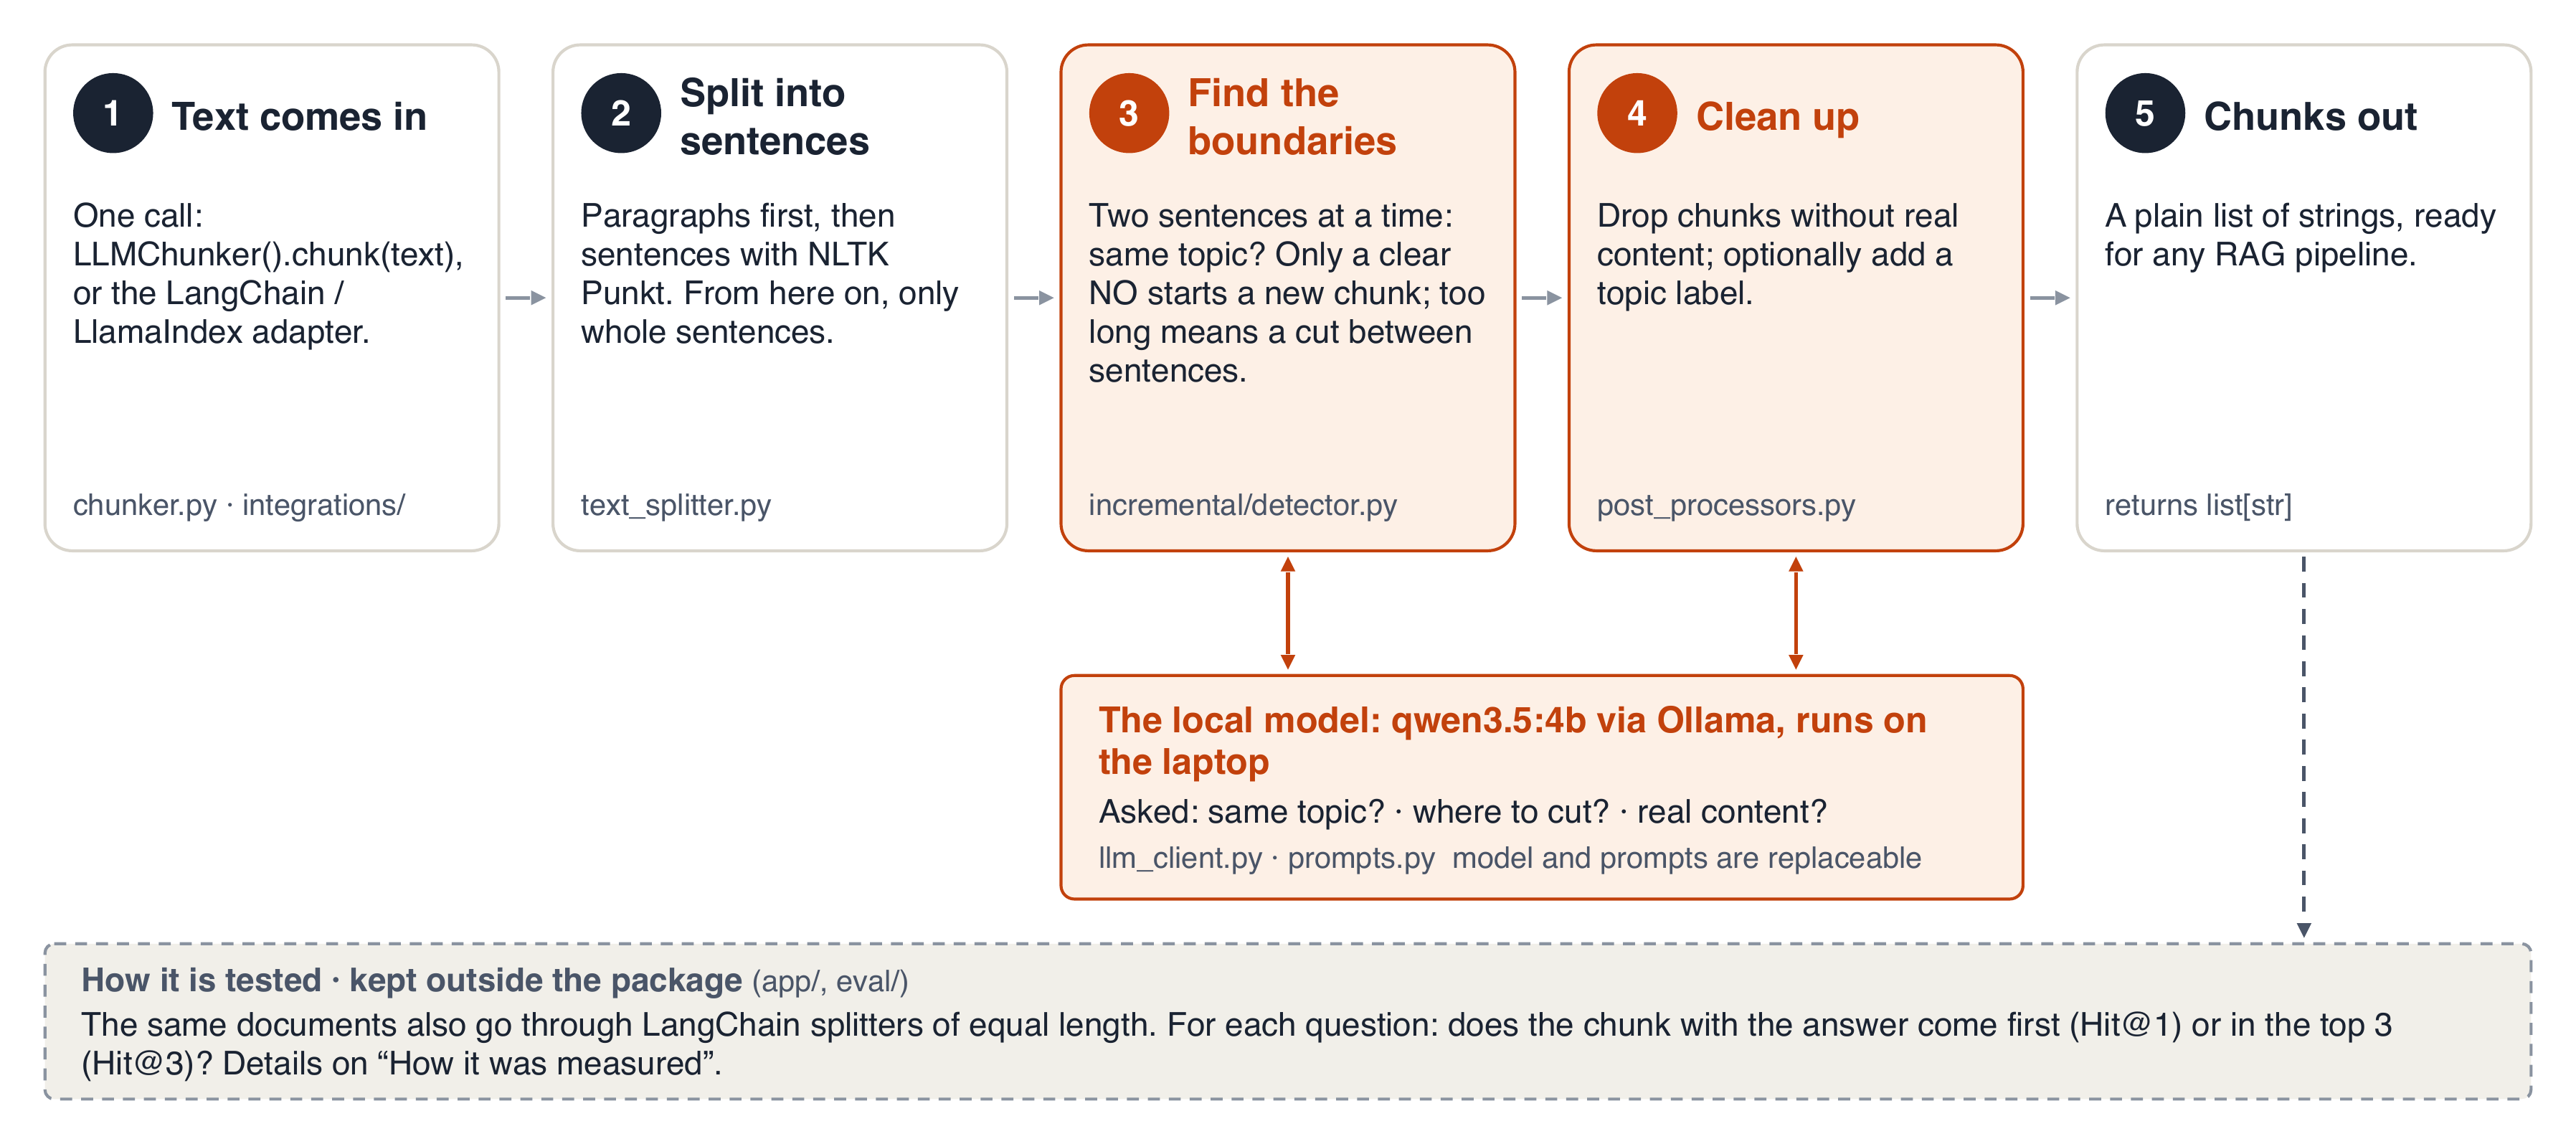
\includegraphics[width=\textwidth]{figures/architecture.png}
  \caption{Architecture of the library. A document passes five stages; the local
  model is asked during boundary detection (step 3) and by the optional
  post-processors (step 4). The evaluation harness is kept outside the package.}
  \label{fig:pipeline}
\end{figure}

\subsection{Boundary detection and size cap}
\label{sec:impl-incremental}
\label{sec:impl-sizecap}

The LLM-based chunking rests on two principles. First, the decision whether a sentence
belongs to the current chunk is \emph{incremental}: the model never sees the whole
document, only the current chunk and the next few sentences. This keeps every LLM call far
below the context window (4096 tokens by default) and makes the cost linear in the
document length. Second, merging is implicit: sentences are joined into chunks while the
model moves through the document, not in a separate step afterwards. \Cref{lst:loop} shows
the core of the loop.

\begin{lstlisting}[caption={The assembly loop, condensed.},label={lst:loop}]
while pos < len(sentences):
    candidate = sentences[pos:pos + self.step_sentences]
    pos += self.step_sentences

    if not current:                                  # first group of a chunk
        current = list(candidate)
    elif self._same_topic(current, candidate, pos):  # one LLM call
        current.extend(candidate)
    else:                                            # topic boundary
        chunks.append(" ".join(current))
        current = list(candidate)

    while self._over_limit(current):                 # size cap, see below
        idx = self._fit_split(current)
        chunks.append(" ".join(current[:idx]))
        current = current[idx:]
\end{lstlisting}

The condition for closing a chunk and starting a new one is deliberately conservative.
Only an explicit NO from the model sets a boundary; an unclear answer continues the
current chunk. The reason is that, because the process is incremental, a wrong split
cannot be repaired later, whereas a missed boundary merely produces a longer chunk.

The topic decisions alone put no upper limit on chunk length: a twenty-page document about
one subject would in theory become a single, unusable chunk. The settings
\code{max\_chunk\_sentences} and \code{max\_chunk\_chars} therefore force a split once a
chunk exceeds either threshold, regardless of the topic.

Two policies decide where this cut is made, and both cut only between sentences. With
\code{smart\_split}, the default, the model reads the over-long chunk and chooses the
sentence at which the split fits best; the chunker then moves this index backwards until
the first piece fits the character cap. With \code{smart\_split} disabled, the oversized
chunk is cut at its middle sentence. The two policies form one of the ablations in
\cref{sec:ablations}: they differ only in where the cap cuts, not in whether it applies.

The size cap is a target, not a guarantee. Because cuts are only made at sentence
boundaries, a single sentence that is longer than \code{max\_chunk\_chars} is never split
and becomes a chunk that exceeds the cap.

\subsection{Heading awareness and post-processing}
\label{sec:impl-headings}
\label{sec:impl-postproc}

In addition to the topic decisions, the library can force a boundary at headings, a
feature that was added during the evaluation. It implements three ways of finding
headings. The default mode \code{"regex"} applies a fixed pattern for numbered and named
headings to the sentences after tokenisation. Its successor, the mode \code{"lines"},
works on the raw text before tokenisation and catches headings such as \code{3.2. Error
Handling} that the sentence tokeniser would otherwise break apart. The mode
\code{"hybrid"} additionally asks the model about short sentence groups that the pattern
did not flag, which makes it possible to measure the model's contribution to heading
detection.

Two optional post-processing steps run over the finished chunk list: the low-information
filter and the topic enricher. A third one, a merging step, was considered during the
design but became unnecessary, because the incremental mode merges while it moves through
the document and never revisits chunks it has already closed. In the legacy mode
\code{"window"}, a separate merging step caused errors: the pre-split pieces could already
contain different topics, and a wrong merge diluted the chunk.

The \emph{low-information filter} asks the model for each chunk whether it contains
substantive information. Only an explicit NO removes the chunk; the aim is to keep bare
headings, boilerplate lines and similar fragments out of the index. Its effect depends
strongly on the document: manuals and table-heavy texts lose more chunks than continuous
prose such as a non-fiction book.

The \emph{topic enricher} prefixes each chunk with an LLM-generated line
\code{[Topic: \ldots]}, so that a chunk that is taken out of its document and loses its
context still carries a short descriptive label. Enrichment is disabled by default,
whereas the low-information filter is enabled. Their effects are evaluated in
\cref{sec:filter}.

\subsection{Configuration and the LLM client}
\label{sec:impl-client}

All chunker settings are collected in \code{ChunkerConfig}, an immutable dataclass that
validates itself on construction, so that an invalid setting fails before the chunking
starts. The chunker accepts either a configuration object or the individual settings as
keyword arguments, but refuses both at once, since it would be ambiguous which one takes
precedence. The client, \code{OllamaClient}, wraps Ollama's chat endpoint and adds three
mechanisms that make the output reproducible and complete.

\begin{description}
    \item[Deterministic decoding.] The temperature is set to zero and the seed is fixed
    (\code{temperature=0}, \code{seed=42}), so that repeated runs produce identical
    output (\cref{sec:verify-determinism}).

    \item[A prompt-size guard.] Ollama silently truncates a prompt that exceeds
    \code{num\_ctx}, so the model would judge a chunk of which it sees only a part. The
    client therefore estimates the size of each prompt before sending it (four characters
    per token) and refuses a prompt that would exceed \SI{90}{\percent} of
    \code{num\_ctx}, rather than letting a truncated judgement propagate through the
    chunking. A second check reads the token count that Ollama reports back and logs a
    warning when the prompt comes close to the limit.

    \item[Retries.] Server errors (5xx) and transport errors, such as a model reload or a
    dropped connection, are retried with exponential backoff, while client errors (4xx)
    are raised at once.
\end{description}

\section{Developer guide}
\label{sec:developer-guide}

This section is a guide for developers who want to use the library. It covers the
installation, the three ways of calling the chunker (the native API and two framework
adapters) and the extension points.

\subsection{Installation and native API}
\label{sec:install}
\label{sec:native-api}

The library is published on the Python Package Index as
\code{llm-semantic-chunker}\footnote{\url{https://pypi.org/project/llm-semantic-chunker/}}:

\begin{lstlisting}[language=bash,caption={Installing the library and its optional extras.},label={lst:install}]
pip install llm-semantic-chunker
pip install "llm-semantic-chunker[langchain]"     # LangChain adapter
pip install "llm-semantic-chunker[llamaindex]"    # LlamaIndex adapter, Python 3.10+
pip install "llm-semantic-chunker[pdf]"           # PDF text extraction
pip install "llm-semantic-chunker[vectorstore]"   # ChromaDB wrapper
\end{lstlisting}

The base installation brings only the three runtime dependencies named in
\cref{sec:impl-overview} and is sufficient to chunk strings; everything beyond that is an
extra that is installed on demand.

The chunker is meant to be a small component of a larger pipeline. Computing embeddings
in-process with sentence-transformers would have turned an installation of about
\SI{40}{\mega\byte} into one of well over \SI{800}{\mega\byte} and tied every project using
the library to the PyTorch version used here. Delegating the embeddings to a second
Ollama-served model avoids this dependency instead of hiding it behind an optional extra.
It also needs less memory, which was decisive given the hardware constraints described in
\cref{sec:impl-overview}.

Chunking also requires a local Ollama chat model. The default is \code{qwen3.5:4b}, but any
other Ollama model can be set in the client. On its first call, the sentence splitter
downloads NLTK's punkt data once; later runs reuse it.

Once installed, the chunker is called through its native API (\cref{lst:native}).

\begin{lstlisting}[caption={Chunking a string with the native API.},label={lst:native}]
from llm_semantic_chunker import LLMChunker, OllamaClient

chunker = LLMChunker(client=OllamaClient(), max_chunk_chars=1200)
chunks = chunker.chunk(text)          # -> list[str]
\end{lstlisting}

The return value is a plain list of strings. Character offsets, the governing heading and
similar metadata were deliberately left out, because this work is limited to evaluating
whether LLM-based chunking sets better boundaries than the baseline strategies.

\subsection{Framework adapters and extension points}
\label{sec:integrations}
\label{sec:extending}

The frameworks are integrated through adapters, so that an existing splitter can be
replaced without changing the rest of a pipeline (\cref{lst:adapters}).
\code{LLMSemanticSplitter} implements LangChain's \code{TextSplitter} interface, so that
the methods \code{create\_documents()}, \code{split\_documents()} and
\code{transform\_documents()} come from the base class. \code{LLMSemanticNodeParser} does the same for LlamaIndex: it
subclasses the \code{TextSplitter} of LlamaIndex, which is itself a \code{NodeParser}, so
that the method \code{get\_nodes\_from\_documents()} works directly. In both frameworks,
the adapter only implements \code{split\_text()}; everything else is built on top of it.

\begin{lstlisting}[caption={Replacing an existing splitter. Only the constructor
line changes.},label={lst:adapters}]
# instead of: RecursiveCharacterTextSplitter(chunk_size=700, chunk_overlap=50)
from llm_semantic_chunker.integrations.langchain import LLMSemanticSplitter
splitter = LLMSemanticSplitter(max_chunk_chars=1200)
docs = splitter.create_documents([text])        # -> list[Document]

# instead of: SentenceSplitter(chunk_size=700, chunk_overlap=50)
from llm_semantic_chunker.integrations.llamaindex import LLMSemanticNodeParser
parser = LLMSemanticNodeParser(max_chunk_chars=1200)
nodes = parser.get_nodes_from_documents([Document(text=text)])  # -> list[TextNode]
\end{lstlisting}

The LlamaIndex extra requires Python 3.10 or newer, because \code{llama-index-core}
depends on \code{banks}, which annotates fields as \code{Path | None}. This syntax raises a
\code{TypeError} on Python 3.9, which the chunker itself still supports. LlamaIndex is
therefore kept in a separate extra.

Beyond the adapters, the library has three extension points and one deliberate exception.

\paragraph{The language model.} Any object with a \code{chat(messages) -> str} method can
be passed as \code{client}, for example a wrapper around a hosted API or another local
server.

\paragraph{The prompts.} Each kind of model decision has its own prompt class, which can
be extended or replaced through a keyword argument: \code{incremental\_prompt} for judging
topic shifts, \code{low\_info\_prompt} for removing low-information chunks and
\code{enrichment\_prompt} for adding a topic line.

\paragraph{Logging.} All library messages go through the \code{logging} module behind a
\code{NullHandler}, so that the application decides what is shown; \code{verbose=True}
only attaches a console handler to the package logger.

\paragraph{What is not replaceable.} The assembly loop. It defines the LLM-based strategy
itself, and changing it would interfere with the structure of the project.

\section{Evaluation harness and verification}
\label{sec:harness}
\label{sec:testing}

The evaluation harness is configured by a \code{ChunkerConfig} and an \code{EvalConfig}.
\code{Pipeline} takes a document and runs two phases: first chunk and cache, then embed,
retrieve and score. \code{StrategyCollector} assembles the baseline strategies, the LLM
chunker and all ablation arms, each of which differs from the reference configuration in
exactly one setting. Two safeguards keep the cached chunks consistent. First, each arm's
cache name is derived from its configuration, so that a setting and its cached file cannot
drift apart. Second, each cache stores a fingerprint of the code that drew its boundaries,
a hash over the syntax trees of the relevant modules, so that results from different code
versions cannot be mixed.

Two further checks verify the determinism of the library and the validity of the question
sets. The scripts are in the repository under \code{eval/experiments/} and \code{tools/}.

\paragraph{Determinism.}
\label{sec:verify-determinism}
The evaluation relies on the chunking being deterministic. Repeating full chunking runs of
the evaluated documents would have taken days, so \code{run\_determinism.py} tests this on
a shorter document instead: it chunks the document several times with identical settings
and compares a hash over the chunk lists. In three runs, it produced \num{48} chunks each
with a mean length of \num{673} characters, the identical digest and identical boundary
statistics (\num{27} topic decisions, \num{28} size-cap splits, \num{8} heading and \num{9}
end boundaries, counted before the low-information filter).

\paragraph{Question sets.}
\label{sec:verify-questions}
\code{tools/verify\_questions.py} tests every question against its document. The anchor
must occur in the document verbatim after whitespace normalisation and exactly once, it
must be at least 40 characters long, and no anchor may appear twice in a set. All
\num{1483} anchors of the three sets used in \cref{ch:evaluation} pass, with lengths
between \num{60} and \num{297} characters.

\section{Availability and use of AI tools}
\label{sec:ai-usage}
\label{sec:availability}

The source code is available at \url{https://github.com/antunoviic/semantic-chunking}
under the MIT license, and the library is published on PyPI as \pkg{} (version 1.0.2).
Besides the library, the repository contains the evaluation harness, the three evaluated
documents, the question sets and the chunk lists of the evaluated arms, so that the
evaluation of \cref{ch:evaluation} can be repeated without chunking the documents again.

Claude Code, with different Claude models, was used in VS Code as a pair programmer for
the library and the evaluation harness. It wrote and ran most of the evaluation and
analysis scripts and reviewed code and results. It was also used for research for this
thesis, to build tables and figures, for the presentation, and to proofread the text of
this thesis for spelling, grammar and consistency. Furthermore, the question sets of
\cref{ch:evaluation} were generated by an external language model (Claude Sonnet 5) as
part of the method (\cref{sec:questions}). The research methods, the choice of documents
and the design, architecture and implementation decisions were not delegated to AI tools.
Every review finding was checked against the code or measured before it was accepted, and
the main results were recomputed by a second, independent implementation
(\cref{sec:robustness}).
